\newpage
\subsection{Differenzenquotient - MITTLERE Änderungsrate}

\hfill \break
Die Ableitung von f an der Stelle x ist der Anstieg der Tangente an den Graphen von f im Punkt $(x,f(x))$. Zur
Kennzeichnung der Ableitung wird der Funktionsterm mit dem Symbol $f'(x)$ bezeichnet.
Die Ableitung einer Funktion ist selbst wieder eine Funktion= Ableitungsfunktion. Ihr Funktionswert an der
Stelle x ist $f'(x)$.

\begin{itemize}
    \item $f'(x) = 0$: Das bedeutet, dass die Tangente am Graphen an der Stelle x den Anstieg O hat, die
          Tangente ist also parallel zur x-Achse.
    \item $f'(x) > 0$: Das bedeutet, dass die Tangentensteigung positiv ist, der Graph ist monoton steigend an
          der Stelle x.
    \item $f'(x) < 0$: Das bedeutet, dass die Steigung der Tangente negativ ist und der Graph monoton fallend
          an der Stelle x ist.
\end{itemize}

\begin{enumerate}
    \item Konstante Funktionen ($f(x) = d$, $f'(x) = 0$): Der Graph einer konstanten Funktion ist
          eine Gerade, welche parallel zur x-Achse
          verläuft. Die Steigung ist in jedem Punkt x
          gleich Null!
    \item Lineare Funktionen ($f(x) = kx + d$, $f'(x) = k$): Der Graph der linearen Funktion ist eine
          Gerade mit Anstieg k. Die Steigung ist in
          jedem Punkt k!
\end{enumerate}

\hfill \break
Geometrische Interpretation der mittleren Änderungsrate:\\
Aus der Sekante wird eine Tangente. Der Punkt B geht
in Punkt A über, somit wird $\Delta x$ immer kleiner und
kleiner, es geht somit gegen Null $(\Delta x \rightarrow 0)$.

\hfill \break
Anstieg der Kurve in einem Punkt = Steigung der Tangente:\\
$lim_{\Delta x \rightarrow 0}(\frac{f(b)-f(a)}{\Delta x}) = f'(x) = 1$ = 1. Ableitung von f nach x

\hfill \break
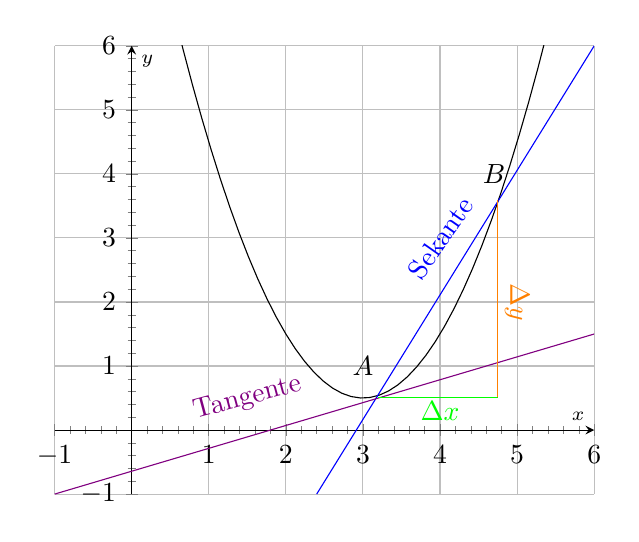
\begin{tikzpicture}[scale=1]
    \begin{axis}%
        [
            grid=major,
            xtick={-1,0,...,7},
            minor x tick num=4, % 4 minor ticks => 5 subintervals
            xmin=-1,
            xmax=6,
            xlabel={\scriptsize $x$},
            axis x line=middle,
            ytick={-1,0,...,7},
            minor y tick num=4,  % 4 minor ticks => 5 subintervals
            ymin=-1,
            ymax=6,
            ylabel={\scriptsize $y$},
            axis y line=middle,
            no markers,
            samples=100,
            domain=-6:6,
        ]
        \addplot[black] (x,{0.5+(x-3)^2});
        \draw[blue] (6,6) -- (2.4,-1);
        \draw[violet] (-1,-1) -- (6,1.5);
        \draw[orange] (4.75,3.6) -- (4.75,0.51);
        \node[color=blue,rotate=55] at (4,3) {Sekante};
        \node[color=violet,rotate=15] at (1.5,0.5) {Tangente};
        \node[color=orange,rotate=-90] at (5,2) {$\Delta y$};
        \draw[green] (3.2,0.51) -- (4.75,0.51);
        \node[color=green] at (4,0.3) {$\Delta x$};
        \node[color=black] at (3,1) {$A$};
        \node[color=black] at (4.7,4) {$B$};
    \end{axis}
\end{tikzpicture}